\documentclass[10pt]{article}

% The automated optical recognition software used to digitize resume
% information works best with fonts that do not have serifs. This
% command uses a sans serif font throughout. Uncomment both lines (or at
% least the second) to restore a Roman font (i.e., a font with serifs).
%\usepackage{times}
%\renewcommand{\familydefault}{\sfdefault}

% This is a helpful package that puts math inside length specifications
\usepackage{calc}
\usepackage{comment}
\usepackage{graphicx}

% Simpler bibsection for CV sections
% (thanks to natbib for inspiration)
\makeatletter
\newlength{\bibhang}
\setlength{\bibhang}{1em} %1em}
\newlength{\bibsep}
 {\@listi \global\bibsep\itemsep \global\advance\bibsep by\parsep}
\newenvironment{bibsection}%
        {\begin{enumerate}{}{%
%        {\begin{list}{}{%
       \setlength{\leftmargin}{\bibhang}%
       \setlength{\itemindent}{-\leftmargin}%
       \setlength{\itemsep}{\bibsep}%
       \setlength{\parsep}{\z@}%
        \setlength{\partopsep}{0pt}%
        \setlength{\topsep}{0pt}}}
        {\end{enumerate}\vspace{-.6\baselineskip}}
%        {\end{list}\vspace{-.6\baselineskip}}
\makeatother

% Layout: Puts the section titles on left side of page
\reversemarginpar

\usepackage[paper=letterpaper,
            %includefoot, % Uncomment to put page number above margin
            marginparwidth=1.2in,     % Length of section titles
            marginparsep=.05in,       % Space between titles and text
            margin=1in,               % 1 inch margins
            includemp]{geometry}

%% Use these lines for A4-sized paper
%\usepackage[paper=a4paper,
%            %includefoot, % Uncomment to put page number above margin
%            marginparwidth=30.5mm,    % Length of section titles
%            marginparsep=1.5mm,       % Space between titles and text
%            margin=25mm,              % 25mm margins
%            includemp]{geometry}

%% More layout: Get rid of indenting throughout entire document
\setlength{\parindent}{0in}

\usepackage[shortlabels]{enumitem}

%% Reference the last page in the page number
%
% NOTE: comment the +LP line and uncomment the -LP line to have page
%       numbers without the ``of ##'' last page reference)
%
% NOTE: uncomment the \pagestyle{empty} line to get rid of all page
%       numbers (make sure includefoot is commented out above)
%
\usepackage{fancyhdr,lastpage}
\pagestyle{fancy}
\pagestyle{empty}      % Uncomment this to get rid of page numbers
\fancyhf{}\renewcommand{\headrulewidth}{0pt}
\fancyfootoffset{\marginparsep+\marginparwidth}
\newlength{\footpageshift}
\setlength{\footpageshift}
          {0.5\textwidth+0.5\marginparsep+0.5\marginparwidth-2in}
\lfoot{\hspace{\footpageshift}%
       \parbox{4in}{\, \hfill %
                    \arabic{page} of \protect\pageref*{LastPage} % +LP
%                    \arabic{page}                               % -LP
                    \hfill \,}}

% Finally, give us PDF bookmarks
\usepackage{color,hyperref}
\definecolor{darkblue}{rgb}{0.0,0.0,0.3}
\hypersetup{colorlinks,breaklinks,
            linkcolor=darkblue,urlcolor=darkblue,
            anchorcolor=darkblue,citecolor=darkblue}

%%%%%%%%%%%%%%%%%%%%%%%% End Document Setup %%%%%%%%%%%%%%%%%%%%%%%%%%%%


%%%%%%%%%%%%%%%%%%%%%%%%%%% Helper Commands %%%%%%%%%%%%%%%%%%%%%%%%%%%%

% The title (name) with a horizontal rule under it
% (optional argument typesets an object right-justified across from name
%  as well)
%
% Usage: \makeheading{name}
%        OR
%        \makeheading[right_object]{name}
%
% Place at top of document. It should be the first thing.
% If ``right_object'' is provided in the square-braced optional
% argument, it will be right justified on the same line as ``name'' at
% the top of the CV. For example:
%
%       \makeheading[\emph{Curriculum vitae}]{Your Name}
%
% will put an emphasized ``Curriculum vitae'' at the top of the document
% as a title. Likewise, a picture could be included:
%
% \makeheading[\includegraphics[height=1.5in]{dering}]{Your Name}
%
% the picture will be flush right across from the name.
\newcommand{\makeheading}[2][]%
        {\hspace*{-\marginparsep minus \marginparwidth}%
         \begin{minipage}[t]{\textwidth+\marginparwidth+\marginparsep}%
             {\large \bfseries #2 \hfill #1}\\[-0.15\baselineskip]%
                 \rule{\columnwidth}{1pt}%
         \end{minipage}}
\newcommand{\Rplus}{\protect\hspace{-.1em}\protect\raisebox{.35ex}{\smaller{\smaller\textbf{+}}}}
\newcommand{\Cpp}{\mbox{C\Rplus\Rplus}\xspace}
% The section headings
%
% Usage: \section{section name}
\renewcommand{\section}[1]{\pagebreak[3]%
    \hyphenpenalty=10000%
    \vspace{1.3\baselineskip}%
    \phantomsection\addcontentsline{toc}{section}{#1}%
    \noindent\llap{\scshape\smash{\parbox[t]{\marginparwidth}{\raggedright #1}}}%
    \vspace{-\baselineskip}\par}

% An itemize-style list with lots of space between items
\newenvironment{outerlist}[1][\enskip\textbullet]%
        {\begin{itemize}[#1,leftmargin=*]}{\end{itemize}%
         \vspace{-.6\baselineskip}}

% An environment IDENTICAL to outerlist that has better pre-list spacing
% when used as the first thing in a \section
\newenvironment{lonelist}[1][\enskip\textbullet]%
        {\begin{list}{#1}{%
        \setlength{\partopsep}{0pt}%
        \setlength{\topsep}{0pt}}}
        {\end{list}\vspace{-.6\baselineskip}}

% An itemize-style list with little space between items
\newenvironment{innerlist}[1][\enskip\textbullet]%
        {\begin{itemize}[#1,leftmargin=*,parsep=0pt,itemsep=0pt,topsep=0pt,partopsep=0pt]}
        {\end{itemize}}

% An environment IDENTICAL to innerlist that has better pre-list spacing
% when used as the first thing in a \section
\newenvironment{loneinnerlist}[1][\enskip\textbullet]%
        {\begin{itemize}[#1,leftmargin=*,parsep=0pt,itemsep=0pt,topsep=0pt,partopsep=0pt]}
        {\end{itemize}\vspace{-.6\baselineskip}}

% To add some paragraph space between lines.
% This also tells LaTeX to preferably break a page on one of these gaps
% if there is a needed pagebreak nearby.
\newcommand{\blankline}{\quad\pagebreak[3]}
\newcommand{\halfblankline}{\quad\vspace{-0.5\baselineskip}\pagebreak[3]}

% Uses hyperref to link DOI
\newcommand\doilink[1]{\href{http://dx.doi.org/#1}{#1}}
\newcommand\doi[1]{doi:\doilink{#1}}

% For \url{SOME_URL}, links SOME_URL to the url SOME_URL
\providecommand*\url[1]{\href{#1}{#1}}
% Same as above, but pretty-prints SOME_URL in teletype fixed-width font
\renewcommand*\url[1]{\href{#1}{\texttt{#1}}}

% For \email{ADDRESS}, links ADDRESS to the url mailto:ADDRESS
\providecommand*\email[1]{\href{mailto:#1}{#1}}
% Same as above, but pretty-prints ADDRESS in teletype fixed-width font
%\renewcommand*\email[1]{\href{mailto:#1}{\texttt{#1}}}

%\providecommand\BibTeX{{\rm B\kern-.05em{\sc i\kern-.025em b}\kern-.08em
%    T\kern-.1667em\lower.7ex\hbox{E}\kern-.125emX}}
%\providecommand\BibTeX{{\rm B\kern-.05em{\sc i\kern-.025em b}\kern-.08em
%    \TeX}}
\providecommand\BibTeX{{B\kern-.05em{\sc i\kern-.025em b}\kern-.08em
    \TeX}}
\providecommand\Matlab{\textsc{Matlab}}

%%%%%%%%%%%%%%%%%%%%%%%% End Helper Commands %%%%%%%%%%%%%%%%%%%%%%%%%%%

%%%%%%%%%%%%%%%%%%%%%%%%% Begin CV Document %%%%%%%%%%%%%%%%%%%%%%%%%%%%

\begin{document}

\makeheading[{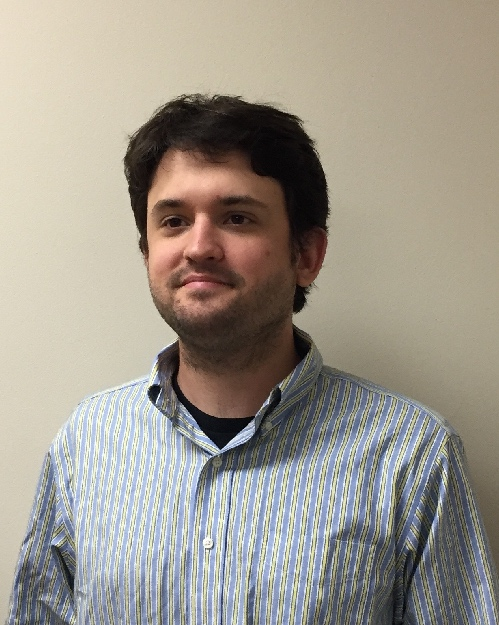
\includegraphics[height=1.2in]{headshot}}]{Matthew L. Dering}

\section{Contact Information}

% NOTE: Mind where the & separators and \\ breaks are in the following
%       table.
%
% ALSO: \rcollength is the width of the right column of the table
%       (adjust it to your liking; default is 1.85in).
%
\newlength{\rcollength}\setlength{\rcollength}{1.4in}%
%
\begin{tabular}[t]{@{}p{\textwidth-\rcollength}p{\rcollength}}
%\href{http://www.cse.osu.edu/}%
%     {Department of Computer Science and Engineering} & \\
%\href{http://www.osu.edu/}{The Ohio State University}
1051 Teaberry Ln, Apt E205  & (610) 209-9072 \\
State College, PA  16803    & \email{matthew.dering@gmail.com}\\
\url{http://sites.psu.edu/dering/} & \\
\end{tabular}

%\section{Objective}

%Insert text here if you want to
%\begin{innerlist}
%\item More information and auxiliary documents can be found at\\\url{http://www.tedpavlic.com/facjobsearch/}
%\end{innerlist}

\section{Research Interests}

Deep Learning, Convolutional Neural Networks, Human Dynamics and Behavior, Product Design, Computer Vision, Automated Content Generation.

\section{Education}

\href{http://www.psu.edu}{\textbf{Penn State University}},
University Park, PA
\begin{outerlist}

\item[] Ph.D.,
        \href{http://www.eecs.psu.edu/}
             {Computer Science and Engineering},
             \emph{Expected:} December 2017
        \begin{innerlist}
        \item Thesis Topic: \emph{Using Deep Learning To Provide Computer Aided Design in Physical Spaces}
        \item Advisors:
              \href{http://www.engr.psu.edu/datalab/people.html}
                   {Conrad S. Tucker, Ph.D} and
              \href{http://www.cse.psu.edu/~duk17/}
                   {Daniel Kifer, Ph.D}
        \end{innerlist}

\item[] M.S.,
        \href{http://www.eecs.psu.edu/}
             {Computer Science And Engineering},
             March 2014
        \begin{innerlist}
        \item Topic: \emph{Android Market: Large Scale Reconstruction and Analysis}
        \item Advisor:
              \href{http://www.patrickmcdaniel.org/}
                   {Patrick McDaniel, Ph.D}
        \end{innerlist}
\end{outerlist}
\vspace{.1in}
\href{http://www.swarthmore.edu}{\textbf{Swarthmore College}},
Swarthmore, PA
\begin{outerlist}
\item[] B.A.,
        \href{http://www.swarthmore.edu/psychology}
             {Psychology} June 2007

\end{outerlist}

\section{Research Experience}

\textbf{Research Assistant} \hfill {July 2014 to present}
\begin{innerlist}

\item[] Penn State DATALab,\\
        Penn State University\\
        Supervisor: Conrad S. Tucker, Ph.D
\end{innerlist}

\textbf{Summer Researcher} \hfill {Summer 2015}
\begin{innerlist}

\item[] Air Force Institute of Technology,\\
        Dayton, OH\\
        Supervisor: Kenneth Hopkinson, Ph.D
\end{innerlist}
\textbf{Research Assistant} \hfill {June 2012 to May 2014}
\begin{innerlist}

\item[] SIISLab,\\
        Penn State University\\
        Supervisor: Patrick McDaniel, Ph.D
\end{innerlist}
\textbf{Summer Intern} \hfill {Summer 2013}
\begin{innerlist}

\item[] Cigital, Inc.\\
        Dulles, VA
\end{innerlist}
\textbf{Summer Student} \hfill {Summer 2012}
\begin{innerlist}

\item[] MIT Lincoln Labs,\\
        Lexington, MA\\
        Supervisor: Thomas Moyer, Ph.D
\end{innerlist}
\textbf{Summer Intern} \hfill {Summer 2011}
\begin{innerlist}
\item[] Cisco Systems,\\
        San Jose, CA
\end{innerlist}


\section{Refereed Publications}
\vspace{-.1275in}
\begin{bibsection}
    \item {\bf Dering, M. L.} and Tucker, C. S. ``Implications of Generative Models in Government'' \emph{AAAI Fall Symposium}, 2017.
    \item {\bf Dering, M. L.}, Tucker, C. S., and Kumara, S.  ``An Unsupervised Machine Learning Approach To Assessing Designer Performance During Physical Prototyping''  \emph{Journal of Computing and Information Science in Engineering}, 2017.
    \item {\bf Dering, M. L.} and Tucker, C. S. ``A Convolutional Neural Network Model for Predicting a Product’s Function, Given Its Form'' \emph{Journal of Mechanical Design: Data Driven Design}, 2017.
    \item {\bf Dering, M. L.} and Tucker, C. S. ``Early Predicting of Student Struggles Using Body Language'' \emph{ASEE Annual Conference \& Exposition}, 2017.

    \item Bodnar, T., {\bf Dering, M. L.}, Tucker, C., and Hopkinson, K. M. ``Using Large-Scale Social Media Networks as a Scalable Sensing System for Modeling Real-Time Energy Utilization Patterns.'' \emph{IEEE Transactions on Systems, Man, and Cybernetics: Systems.}, PP (99):1--14, 2016.
    \item Octeau, D., Jha, S., {\bf Dering, M.}, McDaniel, P., Bartel, A., Li, L., Klein, J. and Le Traon, Y. ``Combining static analysis with probabilistic models to enable market-scale android inter-component analysis.'' \emph{ACM SIGPLAN Notices} 51(1):469--484, 2016.
    \item {\bf Dering, M. L.}, and Tucker, C. S. (2015, August). ``A Computer Vision Approach for Automatically Mining and Classifying End of Life Products and Components.'' \emph{2015 International Design Engineering Technical Conferences and Computers and Information in Engineering Conference} V004T05A007--V004T05A007.
    \item Octeau, D., Luchaup, D., {\bf Dering, M.}, Jha, S., and McDaniel, P. ``Composite constant propagation: Application to android inter-component communication analysis.'' \emph{Proceedings of the 37th International Conference on Software Engineering} 1:77--88, 2015.
    \item {\bf Dering, M. L.}, and McDaniel, P. ``Android market reconstruction and analysis.'' \emph{Military Communications Conference (MILCOM)}, 2014:300--305.
\end{bibsection}

\section{Submitted Conference Publications}
\vspace{-.125in}
\begin{bibsection}
  \item {\bf Dering, M. L.} and Tucker, C. S. ``Generative Adversarial Networks for Increasing the Veracity of Big Data'' \emph{IEEE International Conference on Big Data}, 2017.

\end{bibsection}


\section{Papers in Preparation}
\vspace{-.1in}
\begin{bibsection}
    \item {\bf Dering, M. L.} and Tucker, C. S. ``Dis-Kinect-ed: Using Deep Learning for Simultaneous Pose and Depth Estimation''.
\end{bibsection}

\section{Awards}
Grant Awards
\begin{innerlist}
\item NVIDIA K40 Hardware Grant, June 2016
\end{innerlist}
%
% \halfblankline
%
% Student Awards --- University of Minnesota, Division of Biostatistics
% \begin{innerlist}
% \item Outstanding Teaching Assistant Award\hfill May 2012
% \item Outstanding Research Assistant Award\hfill May 2011
% \item James R. Boen Student Achievement Award\hfill May 2009
% \end{innerlist}
%
% \halfblankline

% Student Awards --- University of Minnesota, Graduate School
% \begin{innerlist}
% \item Doctoral Dissertation Fellowship\hfill 2012--2013
% \begin{innerlist}
%     \item The Doctoral Dissertation Fellowship (DDF) program is intended to give the most accomplished final-year PhD candidates an opportunity to complete the dissertation within the 2012--13 academic year by devoting full-time effort to research and writing.
% \end{innerlist}
% \end{innerlist}

% \section{Presentations}
% Statistical Meetings
% \begin{innerlist}
% \item Workshop on Environmetrics, Raleigh, NC \hfill Oct 2012
% \item Joint Statistical Meetings, San Diego, CA \hfill Aug 2012
% \item Biometric Society (ENAR) Regional Meeting, Washington, D.C. \hfill Apr 2012
% \item Case Studies in Bayesian Statistics and\hfill Oct 2011\\
% Machine Learning, Pittsburgh, PA
% \item Biometric Society (ENAR) Regional Meeting, Miami, FL \hfill Mar 2011
% \item IMS/ISBA Joint International Meeting, Park City, UT \hfill Jan 2011
% \end{innerlist}
%
% \halfblankline
%
% University of Minnesota
% \begin{innerlist}
% \item Mostly Markov Chain Seminar Series \hfill Nov 2011
% \item School of Public Health Research Day \hfill Apr 2011
% \end{innerlist}


\section{Teaching Experience}

%\textbf{Teaching Assistant} \hfill {Springs 2011--12}
% Co-instructor \hfill {Summer 2013}
% \begin{innerlist}
% \item[] PUBH 6400 - Topics in Hierarchical Bayesian Analysis\\
%         with Bradley P. Carlin\\
%         Division of Biostatistics,\\
%         University of Minnesota
% \end{innerlist}

Teaching Assistant \hfill {Fall 2014--Spring 2015}
\begin{innerlist}

\item[] CMPSC 201 - Introduction to Programming for Engineers\\
        Instructor: Martin Yeh, Ph.D\\
        Computer Science and Engineering,\\
        Penn State University
\end{innerlist}

\section{Hardware and Software Skills}
%\begin{comment}
Programming Languages:
%
\begin{innerlist}
    \item Python, C, C\texttt{++}, Java, Ruby, SQL, MySQL, \Matlab, and others
\end{innerlist}
Software:
\begin{innerlist}
  \item Scikit-learn, Tensorflow, Theano, (Py)Torch, Matplotlib, Opencv, PCL, Boost, D3 and many others
\end{innerlist}
Skills:
\begin{innerlist}
  \item Data Science, Robotics, Image Processing, Artificial Intelligence, Text Analysis, Visualization, Time Series Analysis.
\end{innerlist}

\halfblankline
%\end{comment}

\end{document}
